\documentclass[9pt]{article}
\usepackage[margin=1.25in]{geometry}
\usepackage{graphicx}

\usepackage{blindtext}
\title{Hand Gesture Recogntion - Mid Semester Report}
\date{Fall 2020}
\author{Joe Holt, UW-Madison Computer Science}

\begin{document}
\maketitle

\section{Abstract}
For my computer vision project, I am creating an application that can read hand gestures from a webcam stream and make actions (such as changing computer volume) based on those gestures. I have made substantial progress on my project over the past month since the proposal; I have worked to acquire a high quality dataset, built a way to extract features from a webcam stream and finally I built a simple model to test my image pipeline.

\section{Progress}
This section includes information about the progress I have made this far. 

\subsection{Dataset and Data Pre-Processesing}

One of the most time consuming portions of this project so far has been finding a dataset and processing said data so that it can be fed into a model for training and predictions

\subsubsection{Why my initial dataset did not work}

The kinect dataset I talked about in my initial proposal ended up not being ideal for my project. The kinect dataset had 3D and infared data for each image of a handgesture. While the three dimensional data would likely enabled more accurate gesture predictions, I quickly recognized I had no way to generate features for new pictures using just my computer camera system. So, after some searching, I found a new dataset containing typical images: The Kaggle Hand Gesture Recognition dataset \footnote{https://www.kaggle.com/gti-upm/leapgestrecog}. This dataset was much better because it contains normal JPG images with gesture labels, something I can easily generate new feature data for using my cameras on my laptop.

\subsubsection{Processing the Image Data for Training}

Once I had my dataset, I went through the process of processing the training data in such a way that it would work well with a model. Under the system I built, I can easily process new arbitrary images so that they can be ran through the model for prediction. To do this, I set up a system in which when the webcam is first turned on, it takes a picture of the background of the current enviornment (assuming no hands/peopele are in it at the time). After this, the webcam starts reading images and creates masks based on the difference between the origional, hand-free image, and the new web cam image. 

To create the masks, I first convert each image to a gray-scale image. After this, I convert the grayscale image to a binary/logical image by using a binary threshold tool from OpenCV. Finally, I subtract the origional scene from the image with a hand gesture to get a segmented image of just the gesture that will then be feed through my model. 
 
\subsubsection{Example of Processing}

As an example, I have included a look at this process in the image bellow. The first set of images show pictures taken by the webcam. The left most image is the picture of the empty scene, and the two picture to the right show the same scene but with some hand gestures included. The second row of images show the images after converting them to 1 channel images. Finally, the last row shows the masks that are created by subtracting the gestured images from the empty scene. These are the images that will be imported into the model (note: it is not shown here, but these images will be scaled down before passing to the model. I have not made a final decision though on the final size).

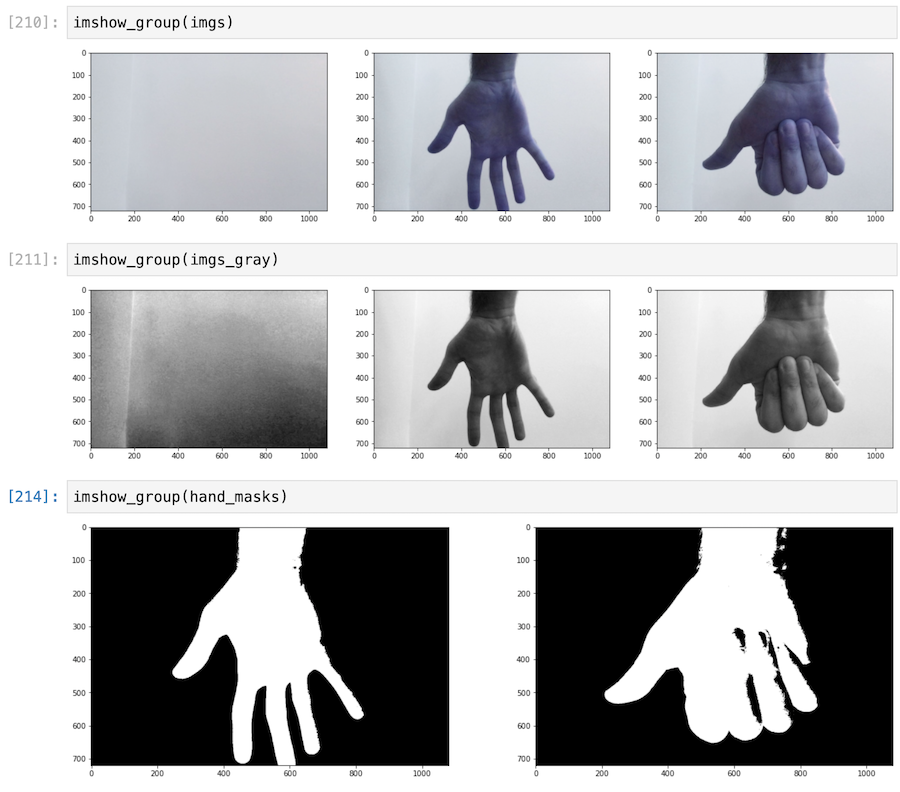
\includegraphics{img_process}

Note: the data in the Hand Gesture dataset I am using comes with the background already segmented out from the hand gestures themselves (the background appears black). Because of this, I am using the exact same image processing steps for these images, minus the "subtracting the background" step (which is replaced with a "subtract black pixels" step).

\subsubsection{Potential Future Work / Issues}
One thing I am worried about with this image processing pipeline is related to the image segmentaion. While the masks that this process creates are relatively good, there are some issues where the mask misses certain parts of the image. For example, the thumbs up in the image above has some areas of the mask missing. I have yet to confirm that this will be an issue, but it is something I am looking out for. Furthermore, there are some gesture classes that are difficult to segment using this method (more on this later).

I have been thinking about adding another processing step that would apply a simple k-means clustering to the masks to further segment them into something that is more realistic. 

\subsection{Model}

I have spent a lot of time getting a simple model working with my pipline. With this in mind, I created a relatively simple CNN model. The model looks somethings like this: input -> conv2d -> maxPool2d -> conv2d -> linear -> linear -> output. I am not going to go into too much detail on the model itself, because it is relatively temporary (I plan to do alot of work on it in the next month).

\subsubsection{Current Results}

After getting the simple model working, I was able to get the following results. The image displays the accuracy across the test dataset for each of the 10 classes in the dataset:

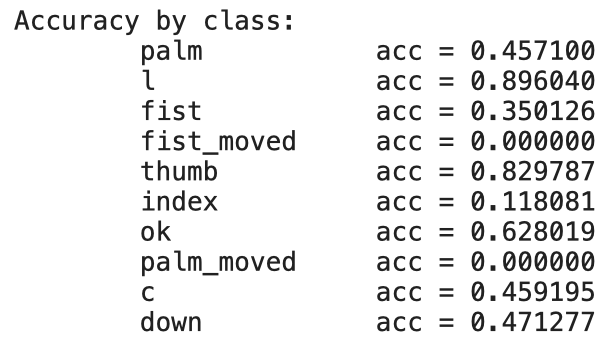
\includegraphics{curr_results}

While these results are not perfect, they are much, much better than randomly guessing a class (which would be ~0.10) for most classes. The only class that the classifier got stuck on is the moving imagry, which it got 0\% on. I believe this is an issue with the way in which I preprocess images rather than the model iteslf.

\subsubsection{Future Work}
As I go forward, I am going to try to refine this model so that I can get higher accuracy accross all classes (especially with the "*\_moved" classes).

\subsection{Application}
Outside of machine-learning/AI portion of this project, I have also made good progress on the application that will utilize my model. This application is a python program that takes over the webcam to capture and segment the enviornment from the gesture in real time.

\subsubsection{Application Running in Static Mode}
The application has a static mode where you can start it by passing an input file and corresponding base image. Under this mode, the app simply predicts for the current image and displays on the screen. An image of this can be seen bellow. Note that the prediction and accuracy is filler data, I do not yet have the model connected.

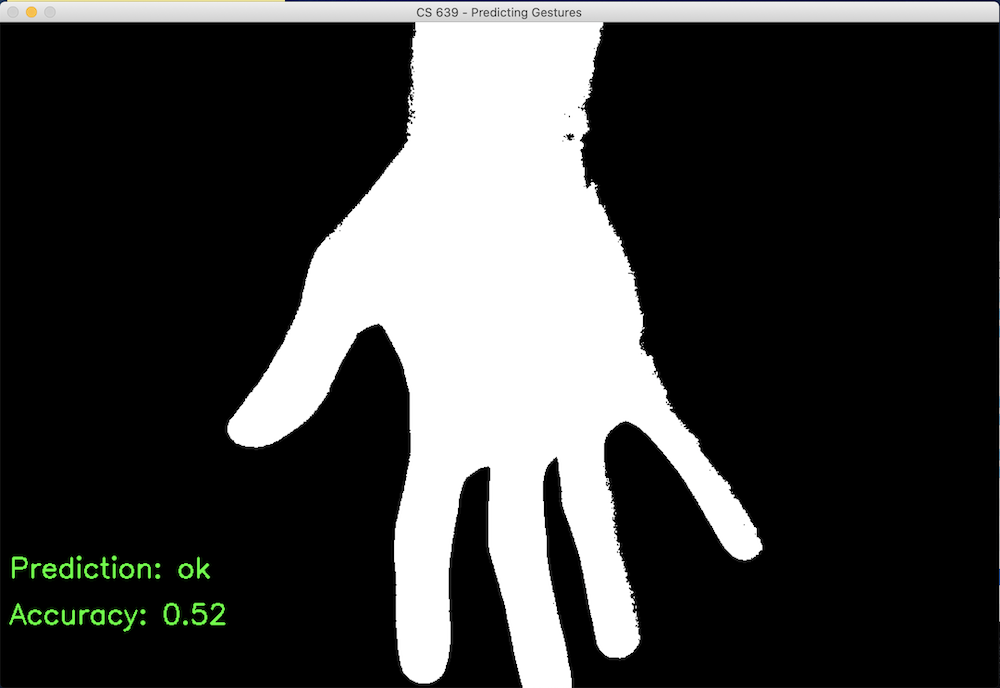
\includegraphics{app_static.png}

\subsubsection{Application Running in Dynamic Mode}
The application also has a "dynamic" mode where it will make preductions from an image stream. When the app is launched in this mode, the first image in the stream is used as the primary background image and is subtracted from subsequant frames to make a mask for the model. I will include an image of what this looks like below. Unfortunately, it works best in a non-noisy enviornment with a solid background color, but I do not have access to that at this moment, which is why the image looks so bad.

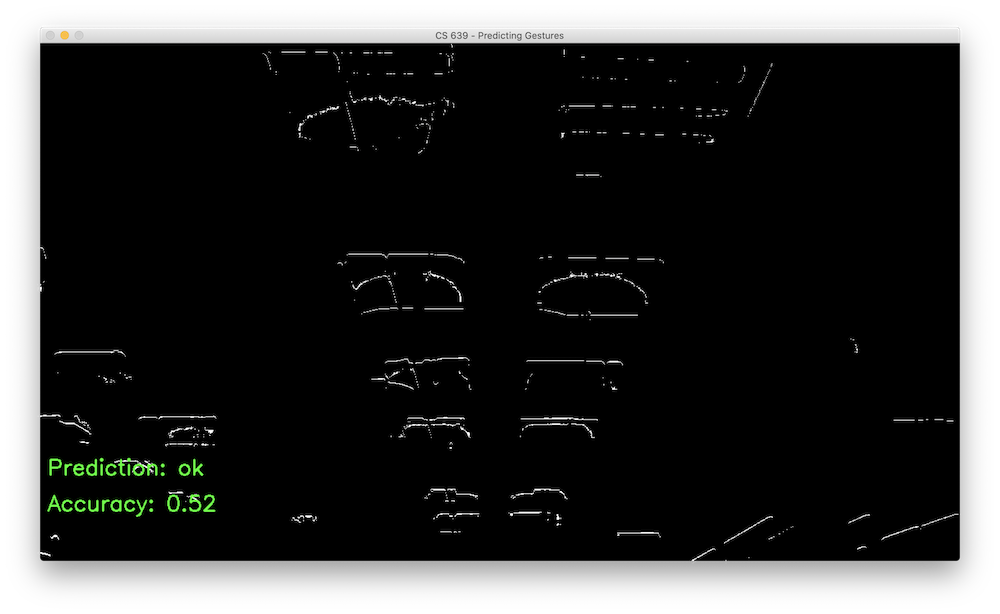
\includegraphics{app_dynamic.png}

\section{Fututre Work}
This section discusses what the next steps are for this project and it lays out what I have to do to complete this project by the deadline.

\subsection{Improving the image processing pipeline}

One of the problems I identified with my current implementation was that the image processing does not work for two classes of moving images (the classes where there is movement with the gesture). Also, I am worried that it is hard for the model to pick out the difference between similar gestures because the image pre-processing removes too many important details.

To fix these issues, I plan on changing my image segmentation policy. To do this, I plan on segmenting my images before I create a mask using a segmentation method we learned about in class: k-Means clustering. 

By segmenting the image via k-Means before appling the binary filter, there will be noise and the segments will be easier to differentiate between one another and the base image. This change will help two fold. First, it will solve our problem of hard-to-differentiate hand gestures because this will increase the amount of detail in my binary masks. Second, I believe this will help us with the moving gestures that had 0\% accuracy in the current build. The reasoning for the low accuracy on these classes is due to poor segmentaiton, so if I improve the segmentation overall, I believe it will be able to better segment moving gestures as well and therefor solve that problem.

\subsection{Improving the Model}

The accuracy on many classes of the model is lower than I would like, and part of the reason is the realtively simple model I am currently using. To improve the accuracy, I am going to attempt to follow two different routes decribed bellow.

\subsubsection{Making my simple model more complex}

I am going to put effort into improving the architecture of my current CNN. I think there alot of areas it could be improved on to improve acurracy. Furthermore, I have not spent addequate time tuning the model and believe I could squeeze some more accuracy out of the model by tuning. 

\subsubsection{Transfer Learning}

I am also going to try using transfer learning to leverage the current (as of April) state of the art model for ImageNet. After some research, I will be attempting to utilize the EfficientNet model\footnote{https://arxiv.org/abs/1905.11946}. This model has provided better results with fewer parameters when compared to other models running against ImageNet. 

By utilizing transfer learning, I will be able to leverage the feature detection and comprehension of the model without the massive training and architecture knowledge cost required to create a similar model by hand. However, I am worried that, dispite not needing to train the entire model, I will still run into issues with not having enough compute power to train the model.

\subsection{Finishing the Application Housing}

The last thing I need to do is to finish the application itself that the model will be built into. This will be realtively quick as I already did a bulk of the work for this step of the project. The following paragraphs explain what is left.

I would like to have the application display N predictions and accuracies where N is the number of predictions with accuracy over 0.50, this change will be relatively quick. 

The biggest change I need to make is the ability to make actions based on the gestures recognized. An action will be executed when the same gesture is recognized with high accuracy (for some definition of high) X times in a row. By the final presentation, the application will be able to increase computer volume if a thumbs up gesture is shown and decrease the volumn if a thumb down gesture is shown.

\section{Conclusion}
Overall I have made a good amount of progress since the proposal, and believe I am on track to complete this project by the deadline. The only issue I forsee causing massive delays is if I run into issues getting my model accuracy up to a sufficient accuracy, but I plan to utilize office hours for help if i get stuck for too long.

\end{document}
